\documentclass[conference]{IEEEtran}
\usepackage{cite}
\usepackage{amsmath,amssymb,amsfonts}
\usepackage{graphicx}
\usepackage{textcomp}
\usepackage{xcolor}
\usepackage{multicol}
\usepackage{float}
\usepackage[spanish]{babel}
\usepackage[spanish,vlined,ruled,]{algorithm2e}

\def\BibTeX{{\rm B\kern-.05em{\sc i\kern-.025em b}\kern-.08em
    T\kern-.1667em\lower.7ex\hbox{E}\kern-.125emX}}
\begin{document}

\title{Imagenes Panorámicas}
\author{\IEEEauthorblockN{Joaquín Pérez Araya}
\IEEEauthorblockA{\textit{Departamento de Ciencias de la Computación} \\
\textit{Universidad de Chile}\\
Santiago, Chile \\
joaquin.perez.a@ug.uchile.cl}}


\maketitle

\begin{abstract}
	El documentó hace referencia al diseño e implementación de la técnica de Stiching, unir dos imágenes por medio de sus similitudes, se usan descriptores locales SIFT para encontrar correspondencias, RANSAC para encontrar una homografía válida y transformar una imagen para calzarla con la otra.
\end{abstract}
 

\section*{Introducción} % ***Así la cosa no me molesta con los numeritos***
	Las imágenes panorámicas actualmente son una variante de fotografías de la mayoría de las cámaras digitales, permiten crear una gran imagen por medio de la toma sucesiva de dos o más fotos que están en la misma escena.
	En análisis de imágenes ésta técnica se llama Stiching, consiste en unir imágenes de una imagen base a otra, a simple vista este proceso podría considerarse trivial, sin embargo se requiere el uso de descriptores locales para encontrar las semejanzas entre las imágenes, algún método estadístico para encontrar un modelo que permita encontrar una transformación adecuada para aplicar a la imagen a unir y finalmente tambien se necesita unir las dos imágenes.
	Para la primera parte de encontrar las semejanzas entre las imágenes, en esta implementación se utilizarán descriptores SIFT cuyo resultado dará pares de puntos que concuerdan entre las dos imágenes.
	Para encontrar la transformación se utilizará el método RANSAC (Consenso de muestras aleatorio, o RANdom SAmple Consensus en inglés), para encontrar una homografía adecuada para llevar a cabo la transformación.
	Para aplicar la transformación se usará interpolación bilineal entre la imagen base y la imagen a transformar.
	
	Como último se utilizará el programa implementado para realizar pruebas utilizando diferentes imágenes y ver el rendimiento del programa creado.
	

\section*{Diseño e Implementación}
	Para el diseño de la implementación se consideran 3 partes distintas, encontrar las concordancias, encontrar la homografía y aplicar dicha homografía:
	\subsection*{Encontrar concordancias}
		Se utiliza la librería OpenCV para utilizar descriptores locales SIFT en las dos imágenes para encontrar concordancias y pares de coordenadas de la imagen base y la imagen de destino. Una vez obtenidas, se verifica que existan al menos 4 pares de puntos para poder calcular la homografía. La implementación que está en el código está fuertemente basada en los ejemplos encontrados en el repositorio del curso.
	\subsection*{Cálculo de Homografía}
		Para el cálculo de la homografía se aplica el método RANSAC que se explica a continuación:
		El método RANSAC funciona de la siguiente forma:
		\begin{itemize}
			\item Elige una pequeña muestra representativa, en este caso 4 pares de puntos: 4 de destino $d$, 4 de fuente $s$.
			\item Con esta muestra, se arma un modelo, en este caso usando los 8 pares de puntos construye una matriz de $9 \times 9$ la cual procede a resolver la ecuación $s  \cdot H = d$, la metodología para la construcción de ésta matriz está en el Anexo.
			\item Con la homografía obtenida al resolver el sistema, ésta se aplica a todos los puntos fuente encontrados utilizando SIFT, y se mide su distancia con los puntos de destino, si la distancia entre éstos puntos está bajo un umbral       (\texttt{DISTANCE\_THRESHOLD} en la implementación), éste se cuenta para validar la homografía como correcta, si al final de el cálculo de distancias la cantidad de puntos está bajo el umbral es menor que un determinado porcentaje de la muestra total (\texttt{INLIER\_THRESHOLD} en la implementación) la homografía se descarta y se repite el proceso.
			\item Este proceso se repite una determinada cantidad de veces (\texttt{RANSAC\_TRIES} en el código) para refinar la homografía encontrada.
		\end{itemize}
		Para la experimentación se utilizaron los siguientes parámetros para RANSAC:
		 \begin{itemize}
		 	\item Umbral de distancia (\texttt{DISTANCE\_THRESHOLD}) 4.
		 	\item Porcentaje de inliers para aprobar (\texttt{INLIER\_THRESHOLD}) $30\%$.
		 	\item Intentos totales (\texttt{RANSAC\_TRIES}) 10.
		 \end{itemize}
	\subsection*{Unión de Imágenes}
		Para unir las imágenes primero se crea un lienzo a partir de la homografía para crear el espacio correspondiente para ubicar las dos imágenes, éste lienzo por defecto tiene el tamaño de ambas imágenes juntas sumadas, en este lienzo posteriormente se procede a copiar la imagen de destino directamente. Luego, se itera por los puntos vacíos del lienzo los cuales se rellenan, si es posible\footnote{La transformación inversa lleva la mayoría de los puntos a lugares que están afuera de la matriz de colores de la imagen fuente} con una interpolación bi-lineal de colores de la imagen de fuente al encontrarse con pixeles.


\section*{Experimentación}
	Para la experimentación se utilizaron imágenes los casos de pruebas pedidos más un caso extra.


\begin{figure}[H]
    \centering
    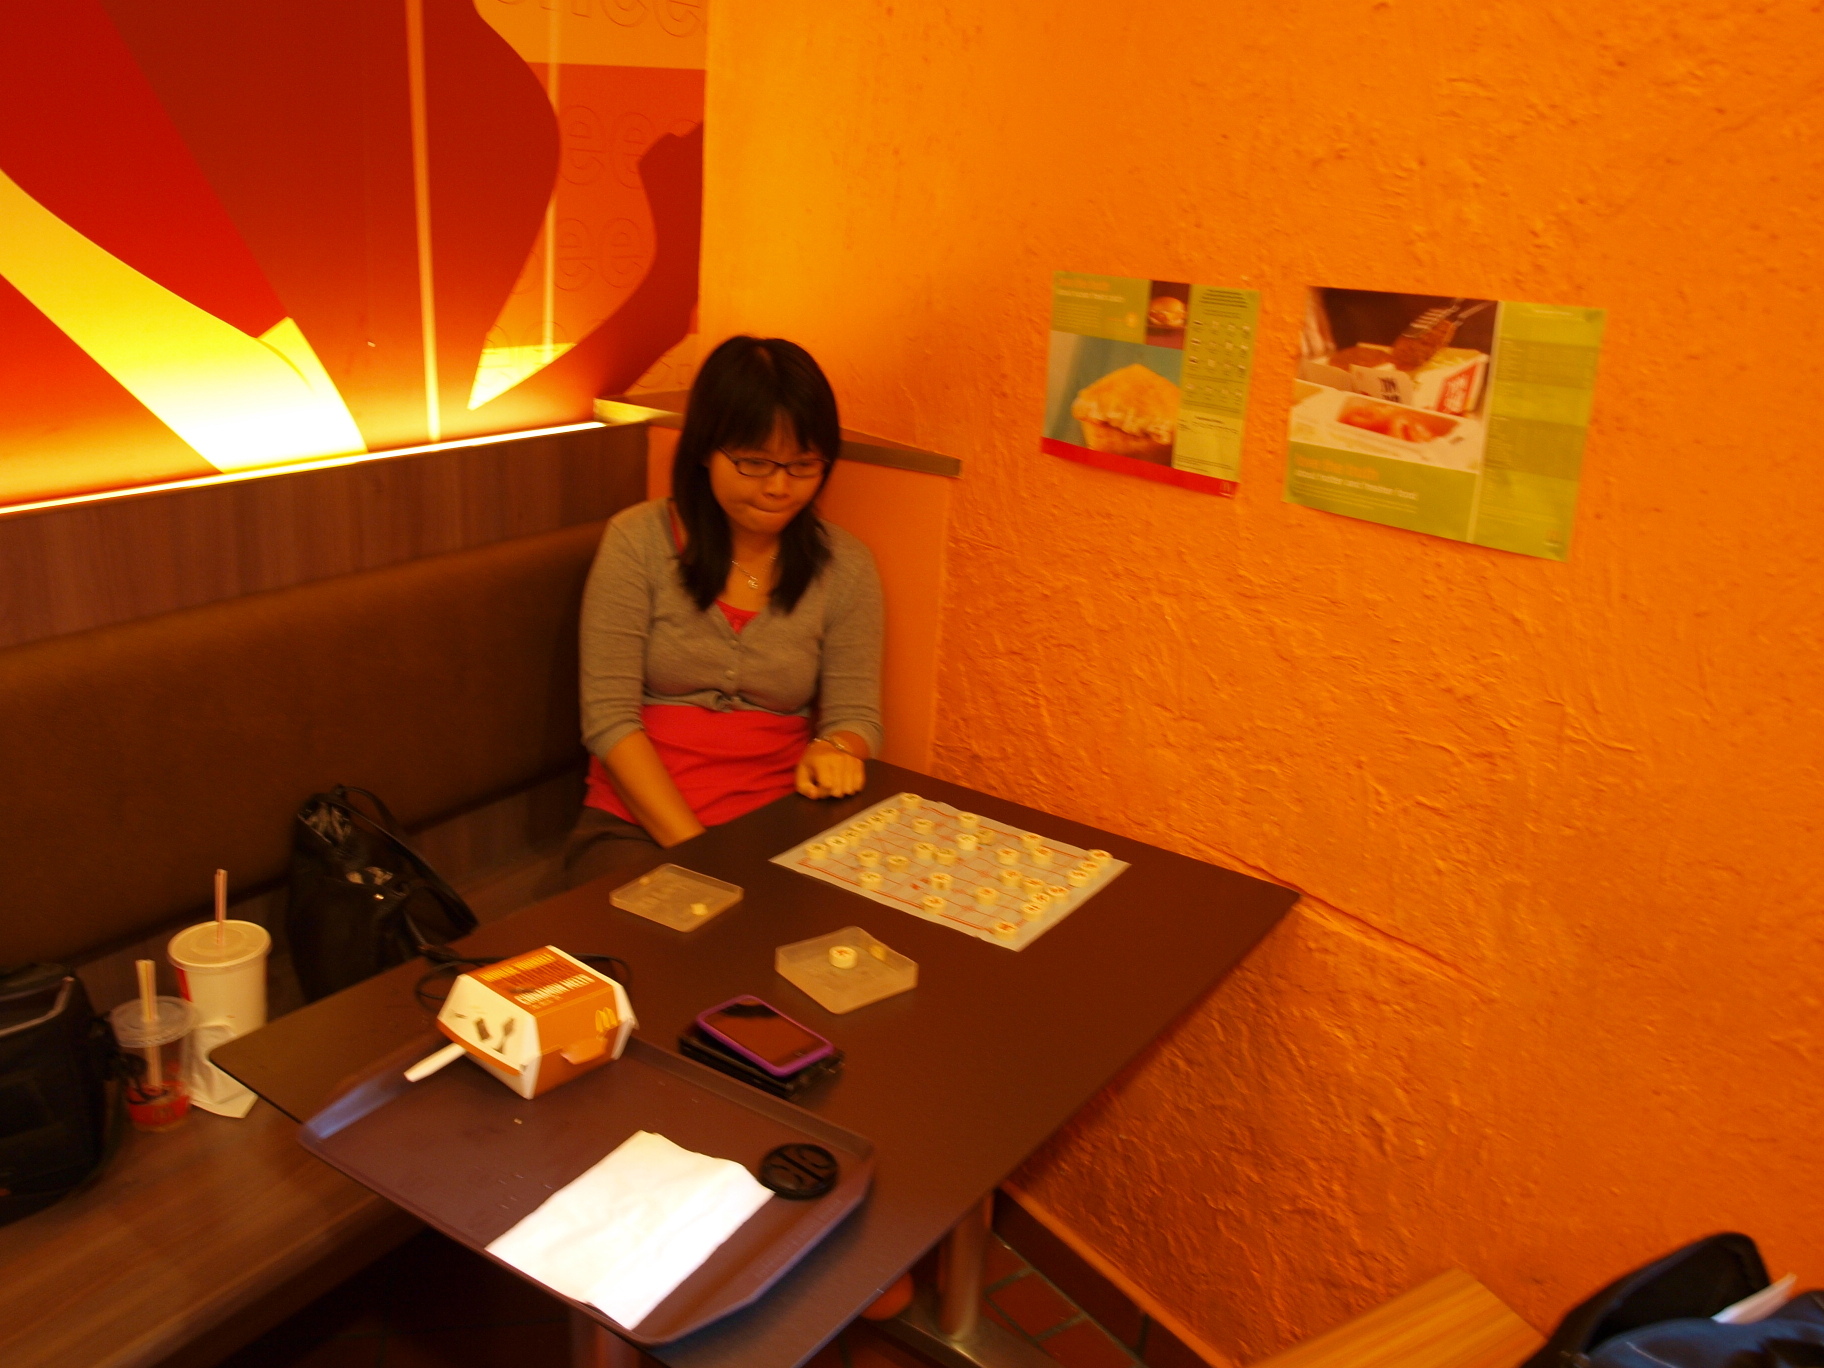
\includegraphics[width=0.80\linewidth]{image/caso_1/1a} \par

\caption{Caso 1: Imagen fuente}
\end{figure}

\begin{figure}[H]
    \centering
   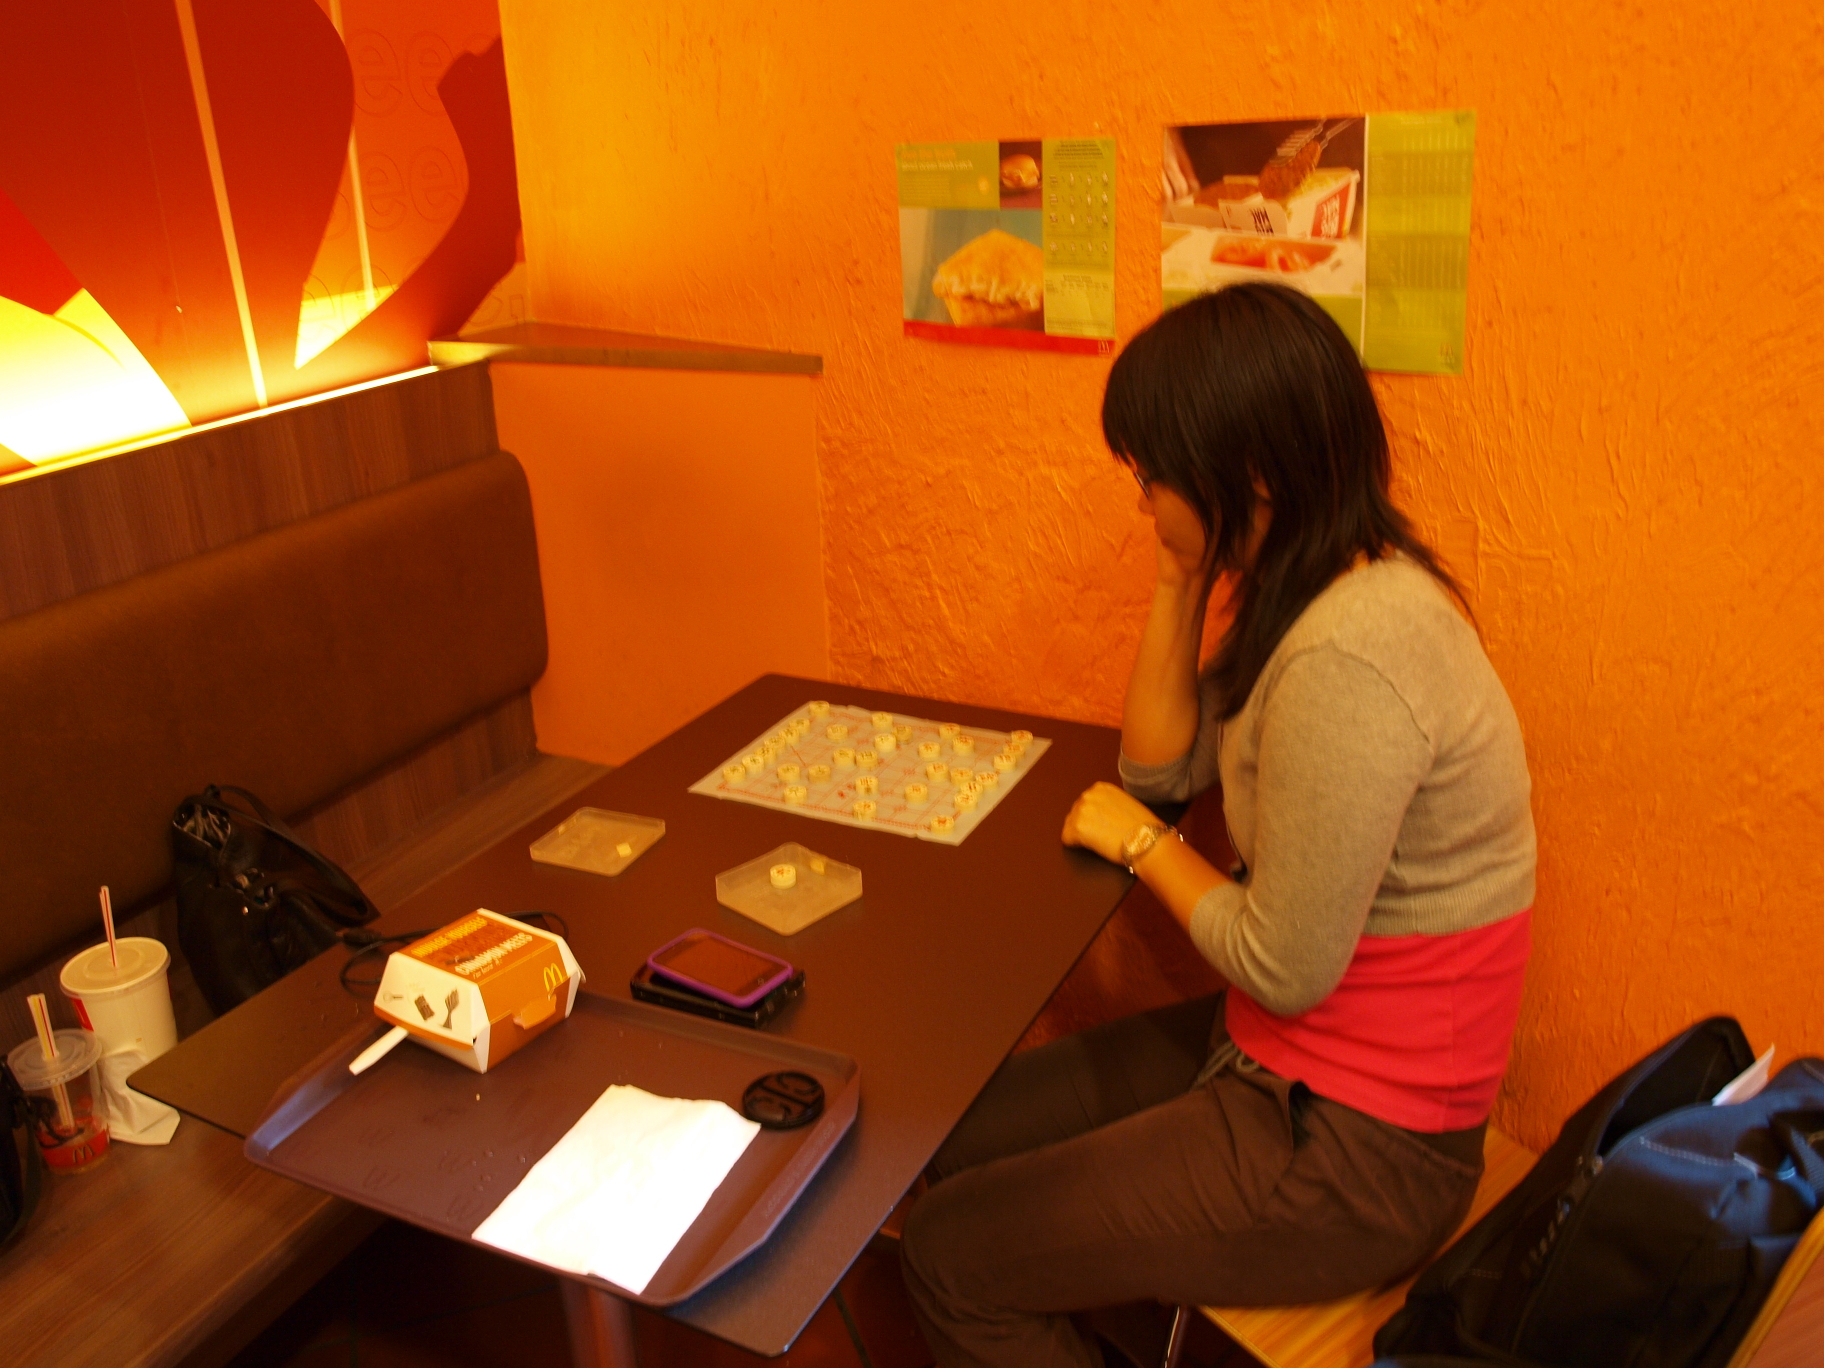
\includegraphics[width=0.80\linewidth]{image/caso_1/1b} \par \par

\caption{Caso 1: Imagen destino}
\end{figure}


\begin{figure}[H]
    \centering
    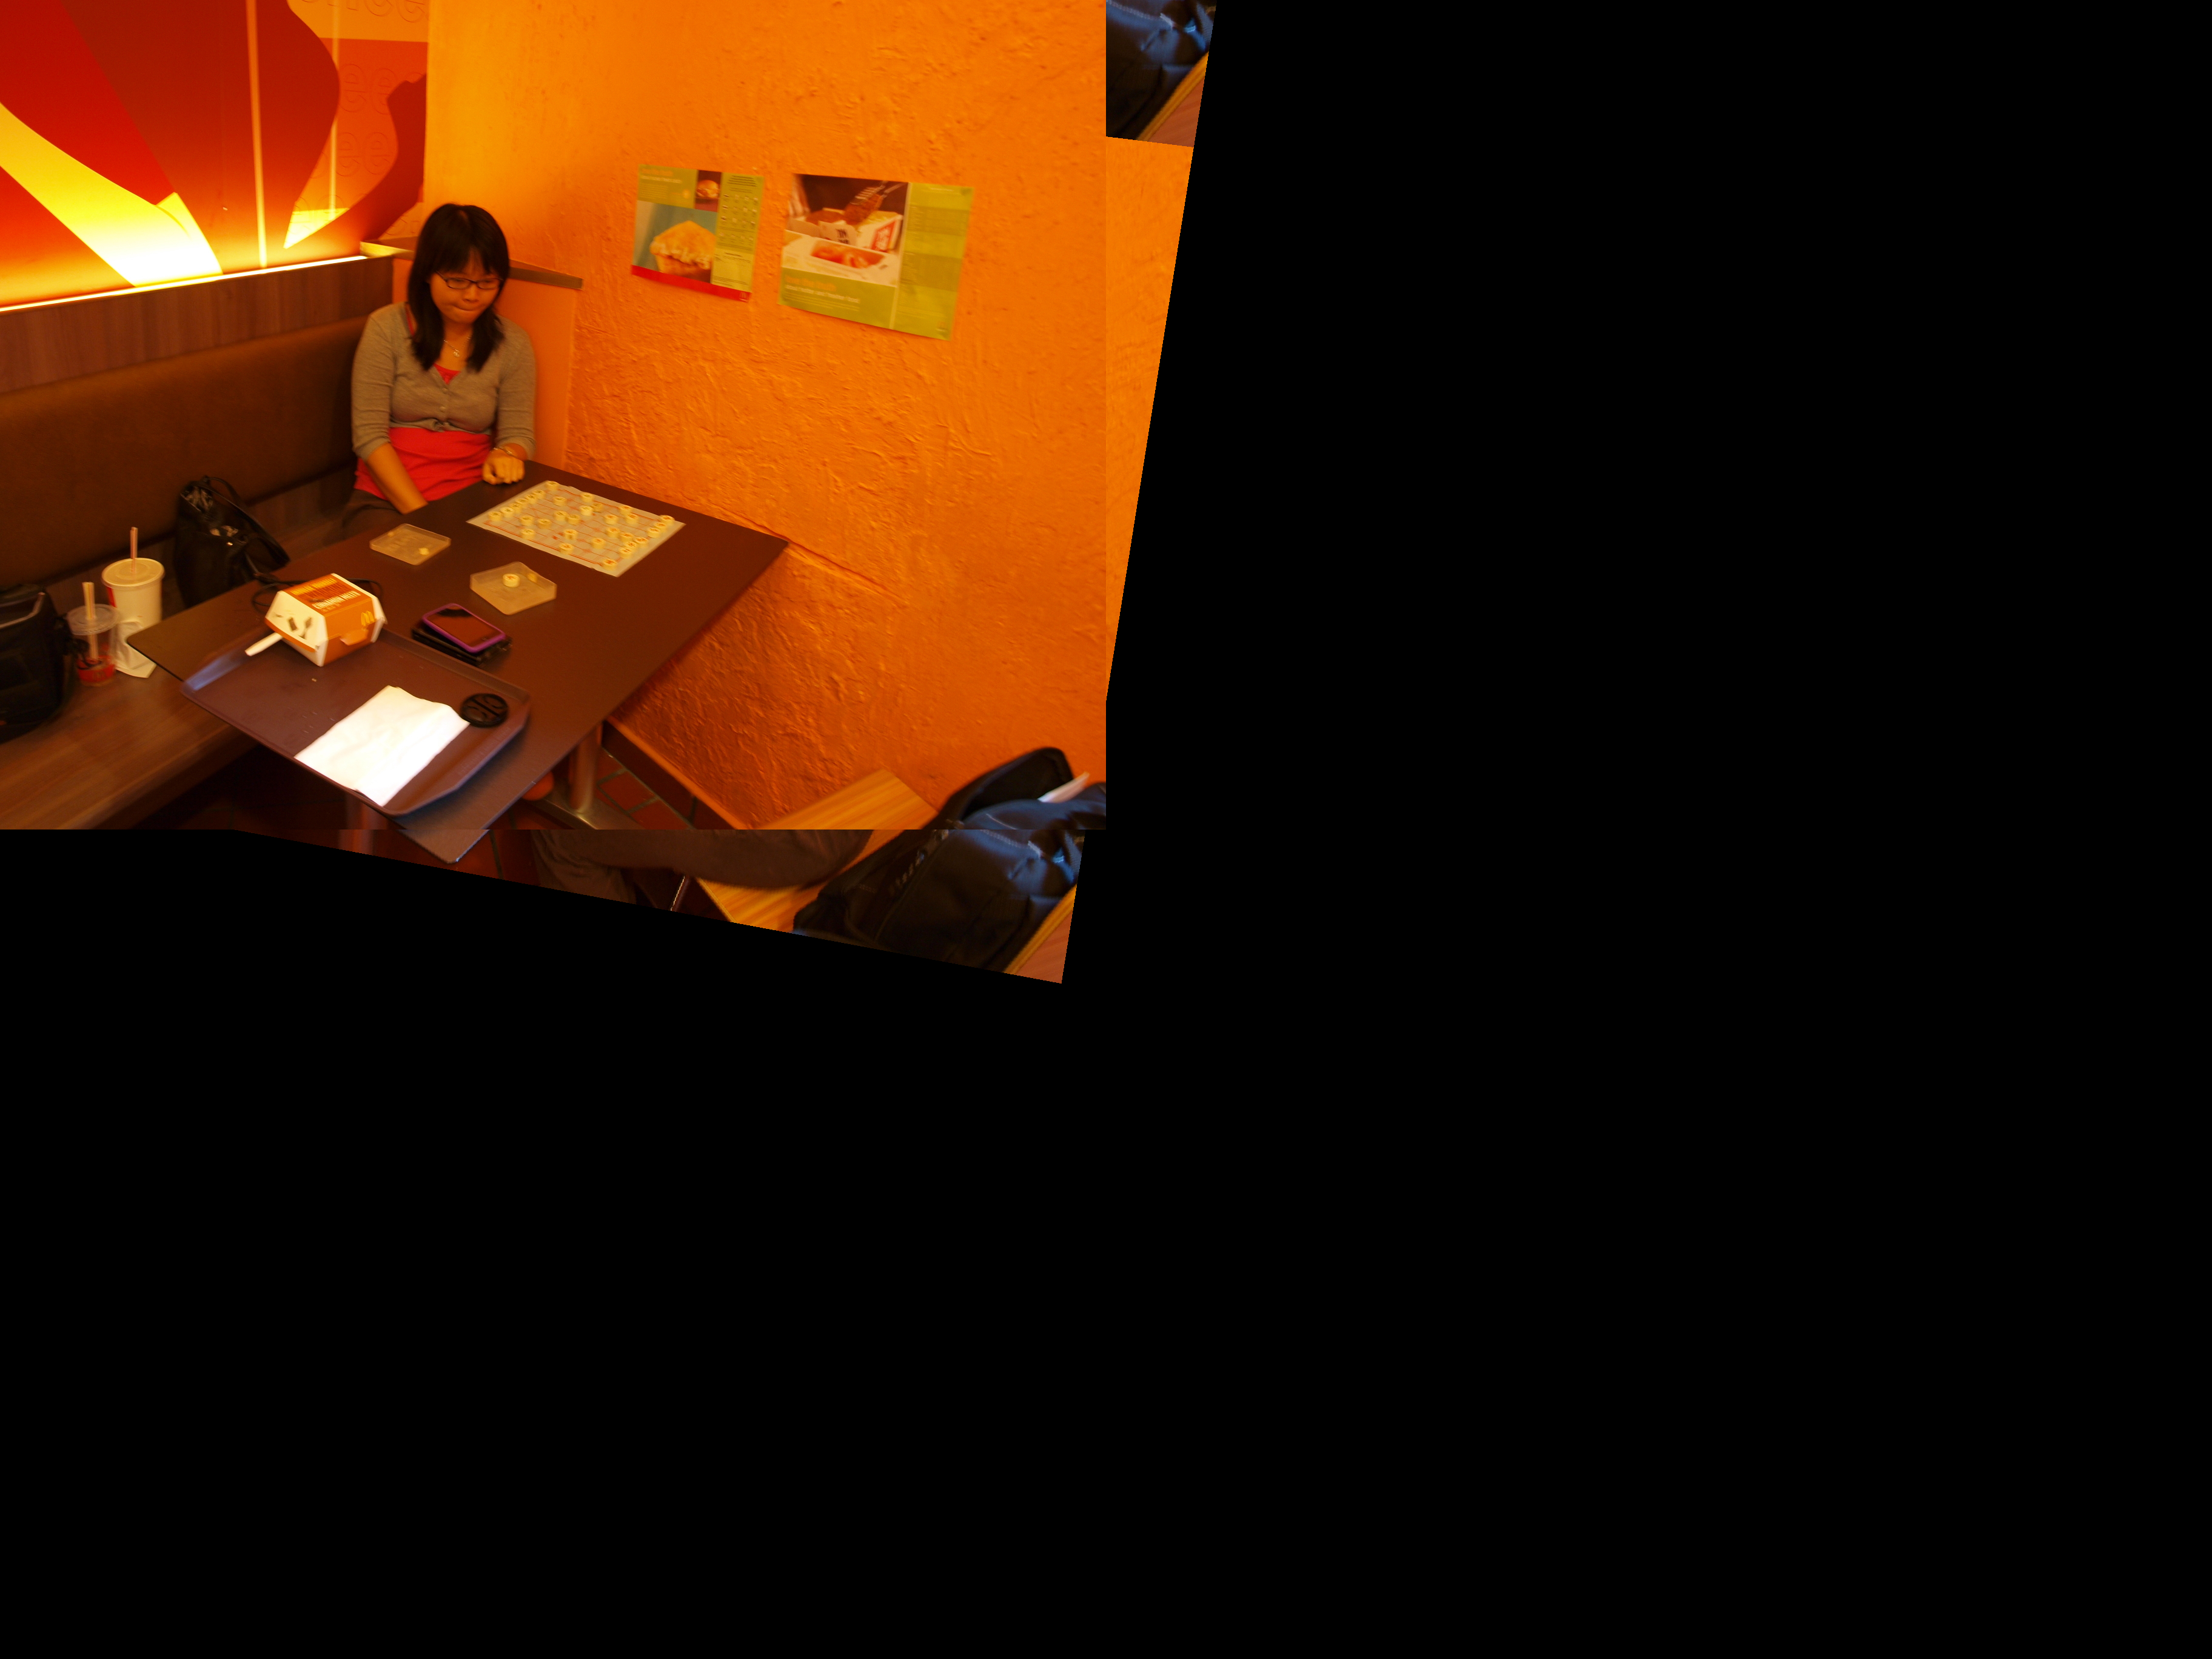
\includegraphics[width=0.95\linewidth]{image/panoramica1.png} \par

\caption{Caso 1}
\end{figure}
	
	En el caso 1, el método falla, quizás sea debido a la orientación de las fotos.


\begin{figure}[H]
    \centering
    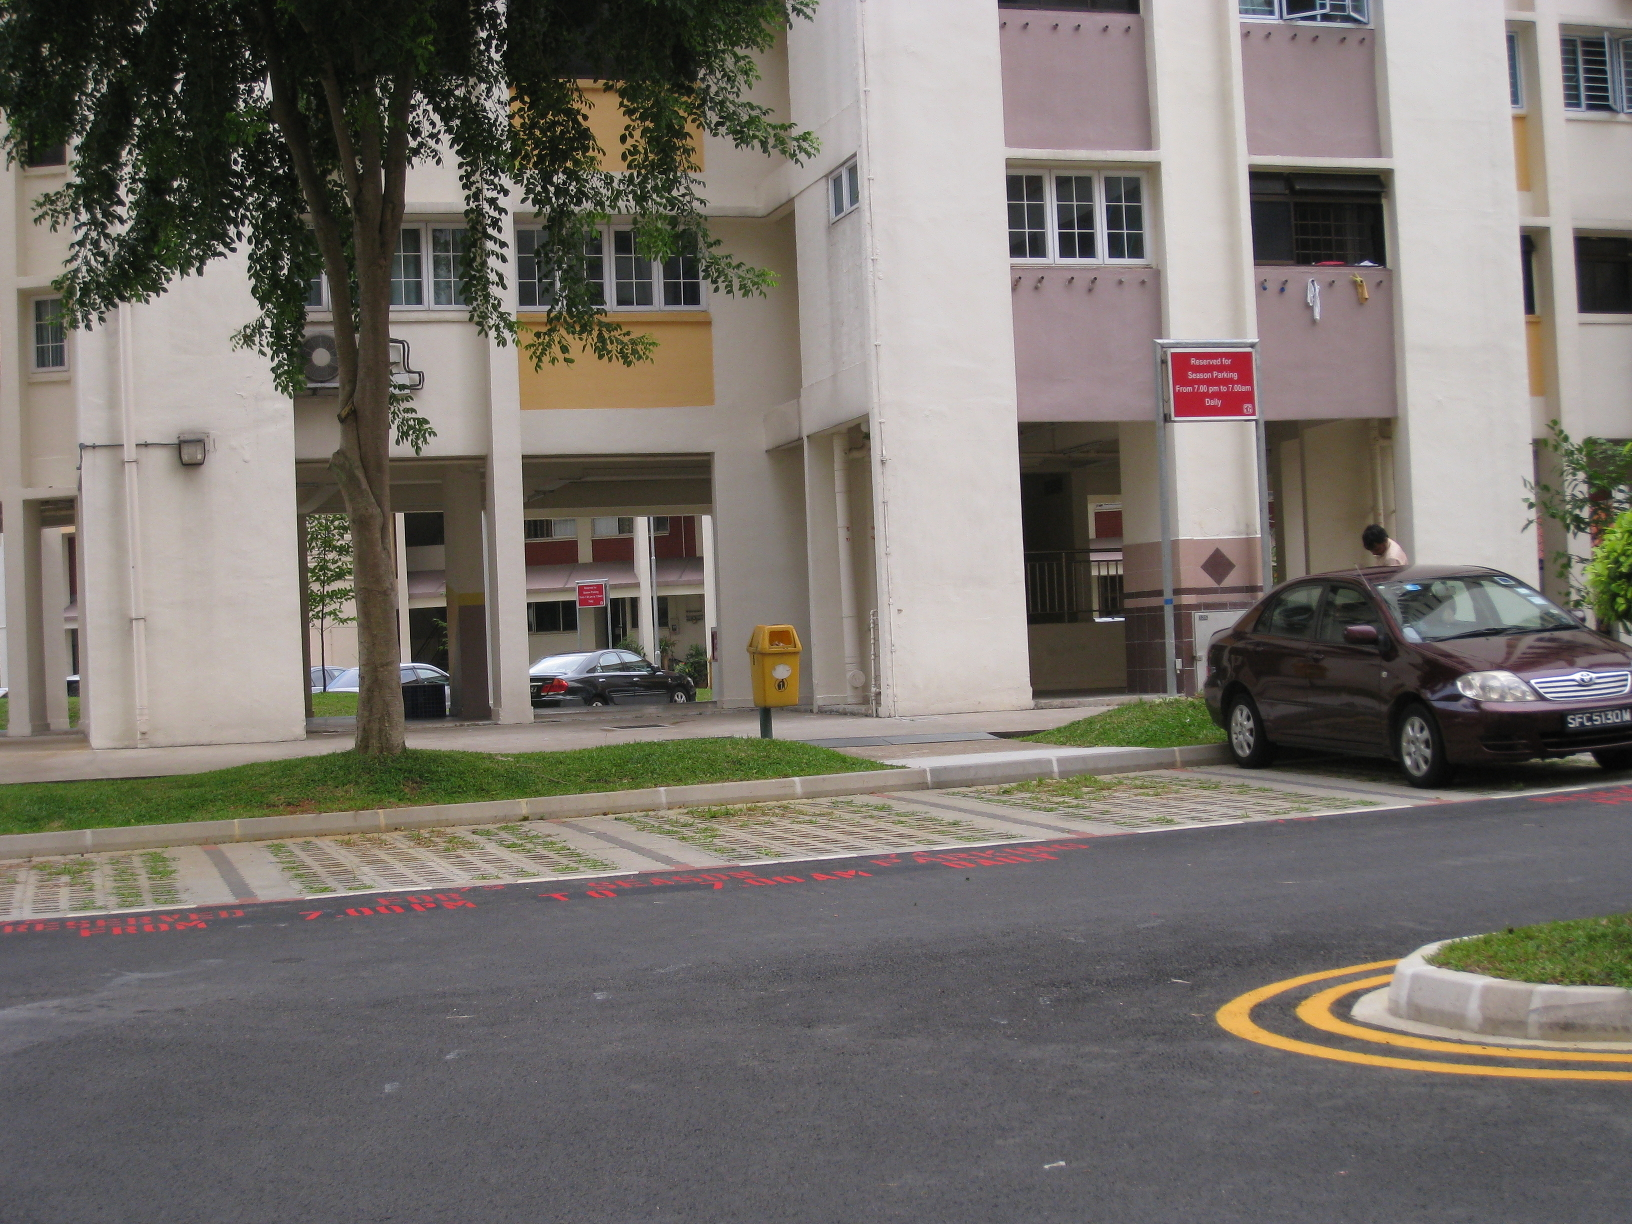
\includegraphics[width=0.80\linewidth]{image/caso_2/2a} \par

\caption{Caso 2: Imagen fuente}
\end{figure}

\begin{figure}[H]
    \centering
   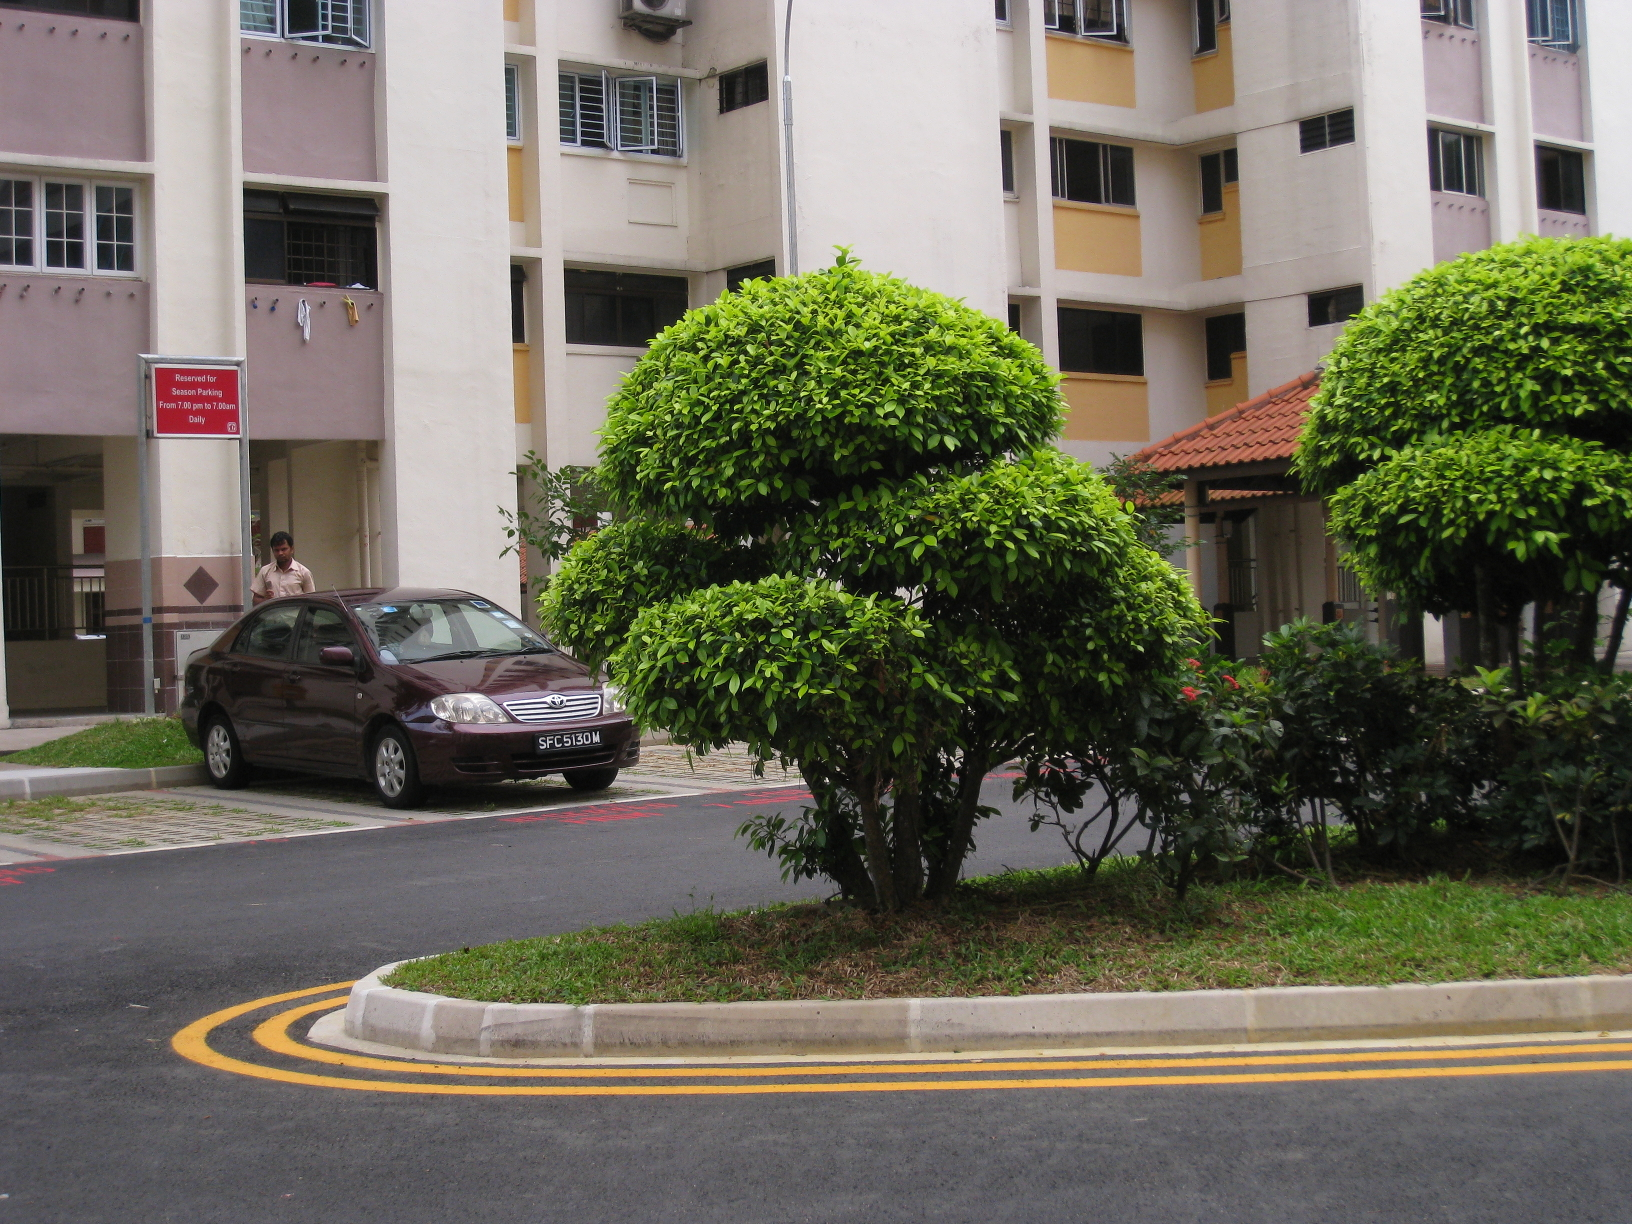
\includegraphics[width=0.80\linewidth]{image/caso_2/2b} \par \par

\caption{Caso 2: Imagen destino}
\end{figure}


\begin{figure}[H]
    \centering
    \includegraphics[width=0.95\linewidth]{image/panoramica2.png} \par

\caption{Caso 2}
\end{figure}

	En el caso 2, la imagen resultante queda casi perfecta enlazada.

\begin{figure}[H]
    \centering
    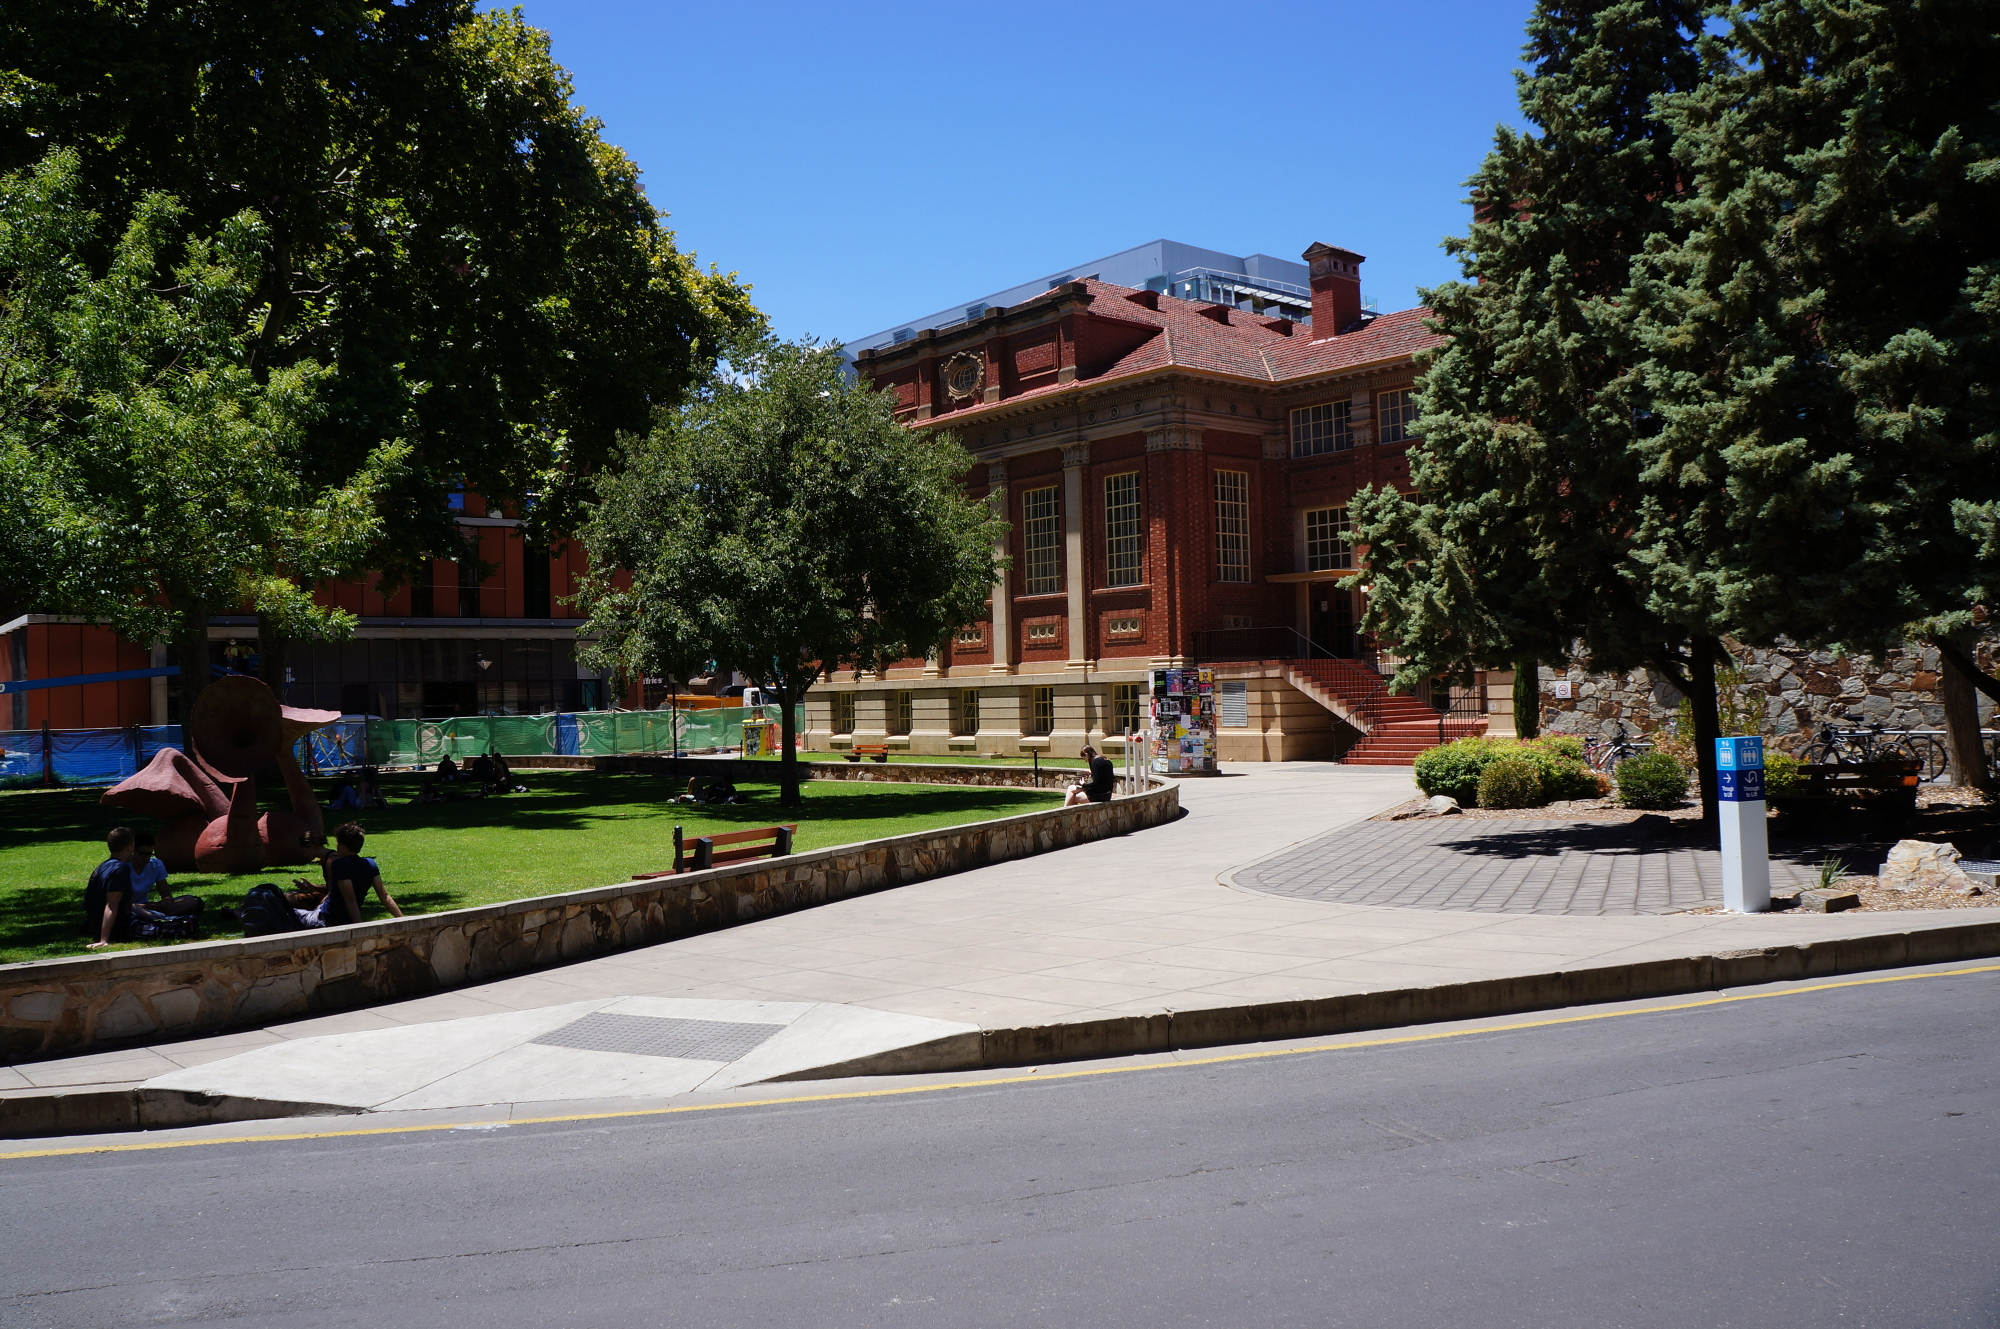
\includegraphics[width=0.80\linewidth]{image/caso_3/3a} \par

\caption{Caso 3: Imagen fuente}
\end{figure}

\begin{figure}[H]
    \centering
   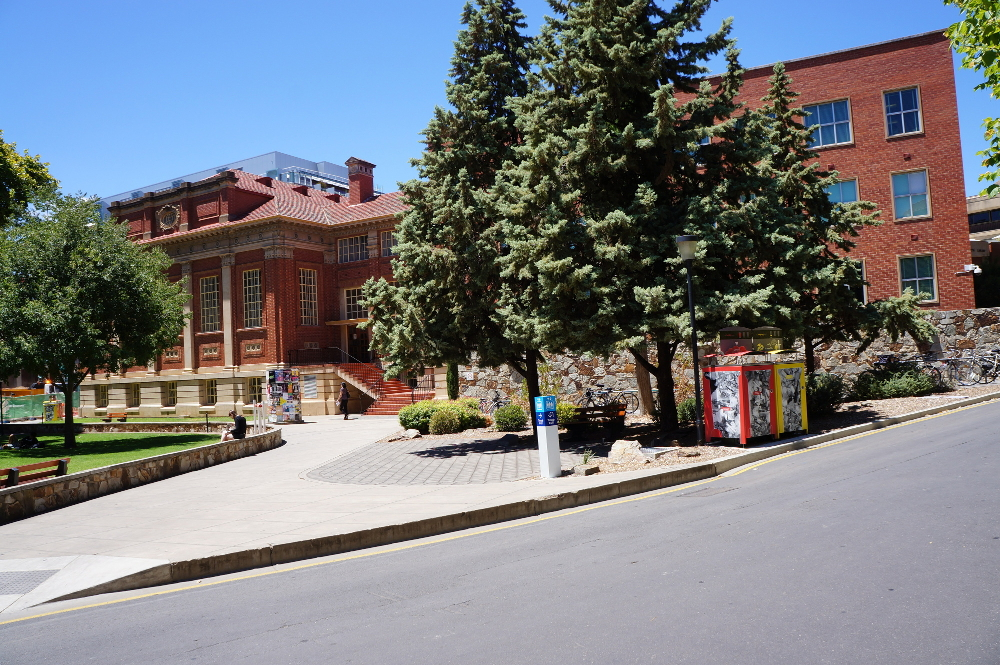
\includegraphics[width=0.80\linewidth]{image/caso_3/3b} \par \par

\caption{Caso 3: Imagen destino}
\end{figure}


\begin{figure}[H]
    \centering
    \includegraphics[width=0.95\linewidth]{image/panoramica3.png} \par

\caption{Caso 3}
\end{figure}
	
	En el caso 3, la imagen resultante está un poco desfasada, especialmente cuando se mira a la línea que forma la vereda.
	
	
	
\section*{Conclusión}
	El método RANSAC permite obtener buenas aproximaciones de homografía, sin embargo su aleatoridad permite que en algunos casos falle completamente o se necesite muchas pruebas para obtener una buena homografía. \\
	La forma de wrapping implementada tampoco no es la mejor, dado que es una mera aproximación, esto causa que el orden el cual se den las fotos al llamar la función \texttt{Panoramic()} sea afectado fuertemente, provocando que falle completamente si las fotos no están ordenadas de izquierda a derecha, por lo que también lo hace más díficil usarlo dado que requiere al menos dos usos para crear una imagen válida.
	

\begin{thebibliography}{99}
	 \bibitem{Caso4} Obtenido de la base de datos \href{www.cvl.isy.liu.se/en/research/datasets/passta/}{LINK}
	 

\end{thebibliography}

\section*{Anexo}
	\subsection{Matriz para resolución de sistemas de ecuaciones.}
		
Sean $p^1, p^2, p^3, p^4$ puntos origen y $q^1, q^2, q^3, q^4$ puntos de destino tal que se cumple para todo punto la siguiente ecuación para la homografía: $p \cdot H = q$, lo que por componente se traduce a: \\
\begin{equation*}
\begin{array}{ccc}
    p_x H_{11} + p_y H_{12} + p_z H_{13} & = & q_x \\
    p_x H_{21} + p_y H_{22} + p_z H_{23} & = & q_y \\
    p_x H_{31} + p_y H_{32} + p_z H_{33} & = & q_z 
\end{array}
\end{equation*}

    Sea $\bar{q}_x = \frac{q_x}{q_z}$, $\bar{q}_y = \frac{q_y}{q_z}$, se divide las dos primeras ecuaciones por $q_z$

\begin{equation*}
    \begin{array}{ccc}
        
    \frac{p_x H_{11} + p_y H_{12} + p_z H_{13}}{q_z} & = & \bar{q}_x \\ 
    
    \frac{p_x H_{21} + p_y H_{22} + p_z H_{23}}{q_z} & = & \bar{q}_y 

    \end{array}    
\end{equation*}    
    
Lo cual es equivalente a:

\begin{equation*}
    \begin{array}{ccc}
    
    \frac{p_x H_{11} + p_y H_{12} + p_z H_{13}}{p_x H_{31} + p_y H_{32} + p_z H_{33}} & = & \bar{q}_x \\
    
    \frac{p_x H_{21} + p_y H_{22} + p_z H_{23}}{p_x H_{31} + p_y H_{32} + p_z H_{33}} & = & \bar{q}_y  \\
    
    \end{array}    
\end{equation*}

Reemplazando ambas equaciones quedan:

\begin{equation*}
    \begin{array}{c}
    
    p_x H_{11} + p_y H_{12} + p_z H_{13} = \bar{q}_x(p_x H_{31} + p_y H_{32} + p_z H_{33}) \\
    
    p_x H_{21} + p_y H_{22} + p_z H_{23} = \bar{q}_y(p_x H_{31} + p_y H_{32} + p_z H_{33})  \\
    
    \end{array}    
\end{equation*}

Reordenando los elementos:

\begin{equation*}
    \begin{array}{c}
    
    p_x H_{11} + p_y H_{12} + p_z H_{13} - \bar{q}_x(p_x H_{31} + p_y H_{32} + p_z H_{33}) = 0 \\
    
    p_x H_{21} + p_y H_{22} + p_z H_{23} - \bar{q}_y(p_x H_{31} + p_y H_{32} + p_z H_{33}) = 0 \\
    
    \end{array}    
\end{equation*}
	Esto equivale a un sistema de dos ecuaciones de la forma:
	\begin{equation*}
	\begin{bmatrix}
	p_x & p_y & p_z & 0 & 0 & 0& -\bar{q}_x p_x & -\bar{q}_x p_y &-\bar{q}_x p_z \\
      0 & 0 & 0 & p_x & p_y & p_z & -\bar{q}_x p_x & -\bar{q}_x p_y &-\bar{q}_x p_z \\
	\end{bmatrix}
		\begin{bmatrix}
		H_{11} \\
		H_{12} \\
		H_{13} \\
		H_{21} \\
		H_{22} \\
		H_{23} \\
		H_{31} \\
		H_{32} \\
		H_{33} \\
	\end{bmatrix}
	= 
		\begin{bmatrix}
		0 \\
		0 \\
	\end{bmatrix}
	\end{equation*}
	Considerando que la coordenada en $z$ no existe dentro de las diferentes imágenes, tomamos $p_z = 1$
	Esta ecuación es válida para los 4 puntos escogidos, por lo que queda un sistema de $8 \times 9$ ecuaciones, para convertir este sistema a uno homogeneo se agrega una ecuación extra $H_{33} = 1$, por lo que el finalmente el sistema de ecuaciones queda:

	\begin{equation*}
	\begin{bmatrix}
	p^1_x & p^1_y & p^1_z & 0 & 0 & 0& -\bar{q}_x p^1_x & -\bar{q}_x p^1_y &-\bar{q}_x p^1_z \\
      0 & 0 & 0 & p^1_x & p^1_y & p^1_z & -\bar{q}_x p^1_x & -\bar{q}_x p^1_y &-\bar{q}_x p^1_z \\

		p^2_x & p^2_y & p^2_z & 0 & 0 & 0& -\bar{q}_x p^2_x & -\bar{q}_x p^2_y &-\bar{q}_x p^2_z \\
      0 & 0 & 0 & p^2_x & p^2_y & p^2_z & -\bar{q}_x p^2_x & -\bar{q}_x p^2_y &-\bar{q}_x p^2_z \\

	p^3_x & p^3_y & p^3_z & 0 & 0 & 0& -\bar{q}_x p^3_x & -\bar{q}_x p^3_y &-\bar{q}_x p^3_z \\
      0 & 0 & 0 & p^3_x & p^3_y & p^3_z & -\bar{q}_x p^3_x & -\bar{q}_x p^3_y &-\bar{q}_x p^3_z \\

	p^4_x & p^4_y & p^4_z & 0 & 0 & 0& -\bar{q}_x p^4_x & -\bar{q}_x p^4_y &-\bar{q}_x p^4_z \\
      0 & 0 & 0 & p^4_x & p^4_y & p^4_z & -\bar{q}_x p^4_x & -\bar{q}_x p^4_y &-\bar{q}_x p^4_z \\
	
	0 & 0 & 0 & 0 & 0 & 0 & 0 & 0 & 1
	\end{bmatrix}
		\begin{bmatrix}
		H_{11} \\
		H_{12} \\
		H_{13} \\
		H_{21} \\
		H_{22} \\
		H_{23} \\
		H_{31} \\
		H_{32} \\
		H_{33} \\
	\end{bmatrix}
	= 
		\begin{bmatrix}
		0 \\
		0 \\
		0 \\
		0 \\
		0 \\
		0 \\
		0 \\
		0 \\
		1 \\
	\end{bmatrix}
	\end{equation*}
	Que se puede resolver como un sistema de ecuaciones lineal.
\end{document}

\begin{figure}[H]
    \centering
    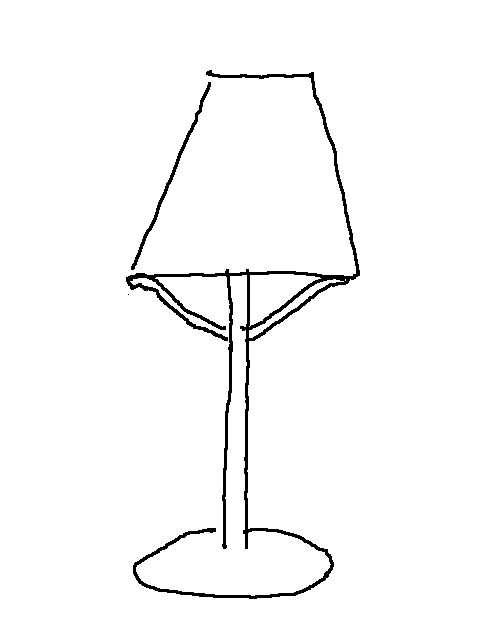
\includegraphics[width=0.95\linewidth]{image/lamps.jpg} \par

\caption{Ejemplo de una posible búsqueda, la imagen de la izquierda representa el dibujo de búsqueda y las de la derecha los resultados esperados.}
\end{figure}